

\documentclass{sig-alternate-05-2015}

% Include useful packages
\usepackage{graphicx}
\graphicspath{ {images/} }
\usepackage{float}
\usepackage{subfig}
\usepackage[table,xcdraw]{xcolor}


\newcommand{\todo}{{\\ \huge \color{red} Still need to do this!!!}} % Inserts Todos Statement

\begin{document}

% Copyright
\setcopyright{acmcopyright}


\title{A Reimplementation of Online Tracking by Learning Discriminative Saliency Map with Convolutional Neural Network}

\numberofauthors{2} 
\author{
% You can go ahead and credit any number of authors here,
% e.g. one 'row of three' or two rows (consisting of one row of three
% and a second row of one, two or three).
%
% The command \alignauthor (no curly braces needed) should
% precede each author name, affiliation/snail-mail address and
% e-mail address. Additionally, tag each line of
% affiliation/address with \affaddr, and tag the
% e-mail address with \email.
%
% 1st. author
\alignauthor
Aaron Gonzales\\
       \email{gonza647@msu.edu}
% 2nd. author
\alignauthor
Steven MW Hoffman \\
       \email{hoffm470@msu.edu}
}
% There's nothing stopping you putting the seventh, eighth, etc.
% author on the opening page (as the 'third row') but we ask,
% for aesthetic reasons that you place these 'additional authors'
% in the \additional authors block, viz.
\date{25 March 2016}
% Just remember to make sure that the TOTAL number of authors
% is the number that will appear on the first page PLUS the
% number that will appear in the \additionalauthors section.

\maketitle

\begin{figure*}[t]
\centering
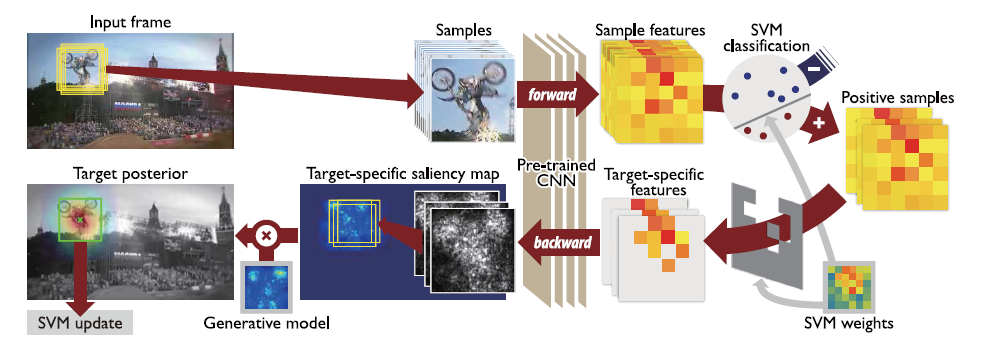
\includegraphics[width=\textwidth]{algorithm}
\caption{A pictoral description of the algorithm described by Hong, et al. in \cite{hong2015online}. Candidate frames are passed through a pre-trained convolutional neural network (CNN) and a feature vector is extracted for each sample from the first fully-connected layer of the CNN. These feature vectors are passed through an SVM, retaining only samples which the SVM believes to contain the target object. The model weights of the SVM are used to determine the target-specific features of each positive sample, which are then back-propagated through the CNN to retrieve a target-specific saliency map. A generative model, produced from previous frames, is convolved with the target-specific saliency map, and the posterior probability that each of the original samples contained the target object is computed.}
\label{fig:algor}
\end{figure*}

\section{Introduction}
We chose to implement our machine learning project with a \textit{deep learning thrust}.
We are basing our project on the work of Hong, et al. \cite{hong2015online}, and our goal is to reproduce their work through the creation of a viable demo.
Hong, et al. propose a novel online tracking scheme for use in applications where tracking an object through frames of a video is desired.
Although there are a large range of potential applications for object tracking software, it is still a difficult problem due to challenges of occlusion, pose variations, illumination changes, fast motion, and background clutter \cite{hong2015online}, and any potential tracking solution must have robust methods to overcome these challenges.
This paper proposes to solve these problems using the combined utility of both a convolutional neural network (CNN) and support vector machine (SVM), wherein a discriminative saliency map is produced and used to calculate the posterior probability of the location of the target in the image.
The object tracking algortihgm by Hong, et al. is described below and is portrayed in Figure \ref{fig:algor}.

The tracking algorithm proposed by \cite{hong2015online} begins by first generating a set of sample images, each of which is drawn from candidate bounding boxes near where the target was located in the previous frame.
Each of these sample images is passed through a pre-trained CNN~\cite{jia2014caffe}.
A CNN is used because CNNs have been shown to be very successful at creating image representations useful for object discrimination.
Additionally, CNNs have shown promise in overcoming challenges from many of the current difficulties presented in object tracking, including pose variations, illumination changes, and background clutter.
For each image, the output from \textit{the first fully-connected layer} of the network is extracted and is used as the feature vector describing that image sample.
The image sample feature vector is then given to an SVM which will classify it as either a positive sample, including the object we are tracking, or a negative sample, which does not include the object we are tracking.
In contrast to the CNN, which is learned offline on generic image data not specific to the target, the SVM is learned online using the samples it has seen up to the previous video frame.
This allows the SVM to adapt to different types of objects which the user would like to track.
For each positive sample, the target-specific features are extracted by using those features which corresponded to positive weights in the SVM, setting all other feature values to zero.
The positive weights of the SVM are chosen because they are the weights which correspond to positively identifying a target.
These target-specific features are then backpropagated through the CNN, producing an image containing a saliency map.
A saliency map is created for every positive sample, and these are combined to make a final target-specific saliency map where larger values in the map indicate a larger likelihood that the target is located at that pixel.
Through these means, the target can be segmented out of the image at a near pixel level.
A generative model is then computed to refine the likelihood estimate based on what has been seen in previous frames.
Finally, the posterior probability of each original sample containing the target is calculated, and the bounding box containing the highest posterior is selected as the target location.
With the target successfully found, the algorithm begins anew in the next frame, creating candidate bounding boxes around where it just found the target in the preceding frame.

\section{Related Work}
The problem of object tracking in video is a large domain, so we will restrict our discussion here to a few works which also attempted to use CNNs to perform tracking, as these are most relevant to the paper we have chosen by Hong, et al. \cite{hong2015online}.
We also highlight how the approach proposed by Hong, et al. differs from these approaches, making it a novel work.

\cite{fan2010human} utilizes a CNN for tracking; however they use an offline trained CNN. They also require a separate class-specific network to track various other objects. Hong, et al \cite{hong2015online}, in contrast, proposes using a pre-trained CNN used for large scale image classification which is trained on generic image data. An online trained SVM is then used in conjunction with the CNN by Hong, et al. to learn the target specific information.

\cite{NIPS2013_5192} also uses a pre-trained network where a stacked denoising autoencoder is trained using a large number of images to learn generic image features. However, as this network is trained on small grey images, its representation power is limited.

\cite{7362006} proposed a target-specific CNN for tracking, where the CNN is trained online. However, this network is shallow in comparison with the deep CNN proposed by \cite{hong2015online}, and as such does not take advantage of the rich information a deep CNN provides.

In addition to the novelties described above, the tracking method proposed by \cite{hong2015online} differs from all three of the above papers in a few important ways.
First, it uses an online trained SVM with the offline trained CNN in order to adapt the tracking to whatever type of object the algorithm happens to be presented with.
Secondly, it uses saliency maps to find the precise location of the tracked object.

\section{Dataset Description}
Following the form of Hong, et al.~\cite{hong2015online}, we tested the tracking algorithm against video sequences from the Tracker Benchmark v1.0 dataset~\cite{wu2013online}. 
This dataset contains 50 testing sequences, i.e. videos containing a specific object to track, all of which vary in video length.
These sequences present a variety of tracking challenges such as illumination variation, deformation, motion blur, background clutter, etc, which can be seen in Table~\ref{tab:vid-attr}.
In addition to these visual challenges, objects of interest vary from humans, to vehicles, to animals, and to various inanimate objects. 
Each of these sequences contain ground truth text files which contain bounding box information for objects of interest at each frame of the video. 
Some of the videos contain multiple objects of interest and as a result come with multiple ground truth files. 
We will analyze our tracking results on these videos qualitatively.
Video frames from a selection of these testing sequences is shown in Figure~\ref{fig:tracker-benchmark}.


% http://www.tablesgenerator.com/ was used to create this table
\begin{table}[]
\centering
\caption{Various video attributes contained within the Tracker Benchmark v1.0 dataset which make objects harder to track in the video. Each of the 50 test videos is annotated with the attributes which that video contains~\cite{wu2013online}.}
\label{tab:vid-attr}
\begin{tabular}{|
>{\columncolor[HTML]{C0C0C0}}c |p{6cm}|}
\hline
\multicolumn{1}{|l|}{\cellcolor[HTML]{C0C0C0}Video Attribute} & \cellcolor[HTML]{C0C0C0}Description                                                                                                                     \\ \hline
IV                                                            & \textit{Illumination Variation}: the illumination in the target region is significantly changed.                                                                 \\ \hline
SV                                                            & \textit{Scale Variation}: the ratio of the bounding boxes of the first frame and,the current frame is out of the range {[}1/ts, ts{]}, ts \textgreater 1 (ts=2). \\ \hline
OCC                                                           & \textit{Occlusion}: the target is partially or fully occluded.                                                                                                   \\ \hline
DEF                                                           & \textit{Deformation}: non-rigid object deformation.                                                                                                              \\ \hline
MB                                                            & \textit{Motion Blur}: the target region is blurred due to the motion of target or camera.                                                                        \\ \hline
FM                                                            & \textit{Fast Motion}: the motion of the ground truth is larger than tm pixels (tm=20).                                                                           \\ \hline
IPR                                                           & \textit{In-Plane Rotation}: the target rotates in the image plane.                                                                                               \\ \hline
OPR                                                           & \textit{Out-of-Plane Rotation}: the target rotates out of the image plane.                                                                                       \\ \hline
OV                                                            & \textit{Out-of-View}: some portion of the target leaves the view.                                                                                                \\ \hline
BC                                                            & \textit{Background Clutters}: the background near the target has the similar color or texture as the target.                                                     \\ \hline
LR                                                            & \textit{Low Resolution}: the number of pixels inside the ground-truth bounding box is less than tr (tr =400).                                                    \\ \hline
\end{tabular}
\end{table}

\begin{figure}[h]
\begin{tabular}{cc}
\subfloat[Deer: MB, FM, IPR, BC, LR]{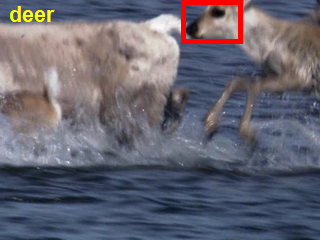
\includegraphics[width = 1.5in]{Deer-ex}}&
\subfloat[MountainBike: IPR, OPR, BC]{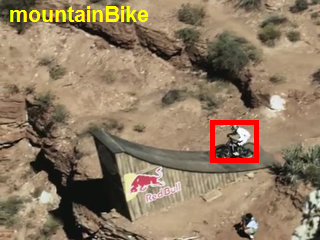
\includegraphics[width = 1.5in]{MountainBike-ex}} \\
\subfloat[Tiger1: IV, OCC, DEF, MB, FM, IPR, OPR]{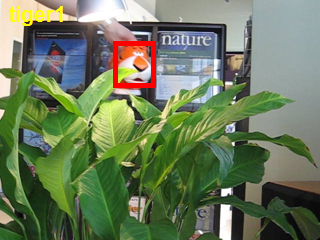
\includegraphics[width = 1.5in]{Tiger1-ex}}&
\subfloat[Walking: SV, OCC, DEF]{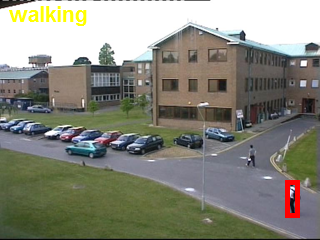
\includegraphics[width = 1.5in]{Walking-ex}} \\
\end{tabular}
\centering
\caption{Video frames from sample sequences in the Tracker Benchmark v1.0 dataset along with bounding boxes drawn around the target object~\cite{wu2013online}. The video attributes are also listed for each shown video.}
\label{fig:tracker-benchmark}
\end{figure}

\section{Tracking Algorithm}
In the introduction, we provided a brief overview of the tracking algorithm proposed by Hong, et al.~\cite{hong2015online}, which we have implemented for our project.
In this section, we will go into more detail describing this algorithm and how we have implemented it.
All of the code for this project was written in Matlab and was executed on both Matlab 2014b and Matlab 2015b.
Note that Figure~\ref{fig:algor} provides a nice pictorial overview of the algorithm.

\subsection{Generating Candidate Sample Patches}
In order to search for the target object in the current frame, candidate sample patches need to be generated, i.e. small portions of the image frame cropped to the size of the target object's initial ground-truth bounding box.
The rest of the tracking algorithm will then be focused on choosing the candidate sample patch, which we will also call a sample or a bounding box, that has the maximum posterior probability of containing the target. 
To generate candidate samples, we first let the bounding box containing the target in the previous frame be a candidate sample for the current frame.
Note that our algorithm will always use the ground truth bounding box provided with the dataset for at least the first frame, beginning tracking with the next frame; this ensures there will always be a bounding box from a previous frame for our algorithm to draw on and it allows us to easily specify which object the algorithm should track in a video by placing the initial bounding box over that object.
We then generate 120 additional samples by drawing from a normal distribution defined by $x_i \sim \mathcal{N}(x_{t-1}^*,\sqrt{wh}/2)$, where $w$ and $h$ denote the width and height of the target bounding box in the initial frame, $x_{t-1}^*$ is the location of the target in the previous frame, and $x_{i}$ is the $i$th sample generated at frame $t$, the current frame. 
This is the same procedure as used by~\cite{hong2015online}, and it is based on the assumption that the most likely locations for the object are distributed around the location of the object in the previous frame.
An example of some of these samples is shown in Figure~\ref{fig:patches}.

\begin{figure}[h]
\centering
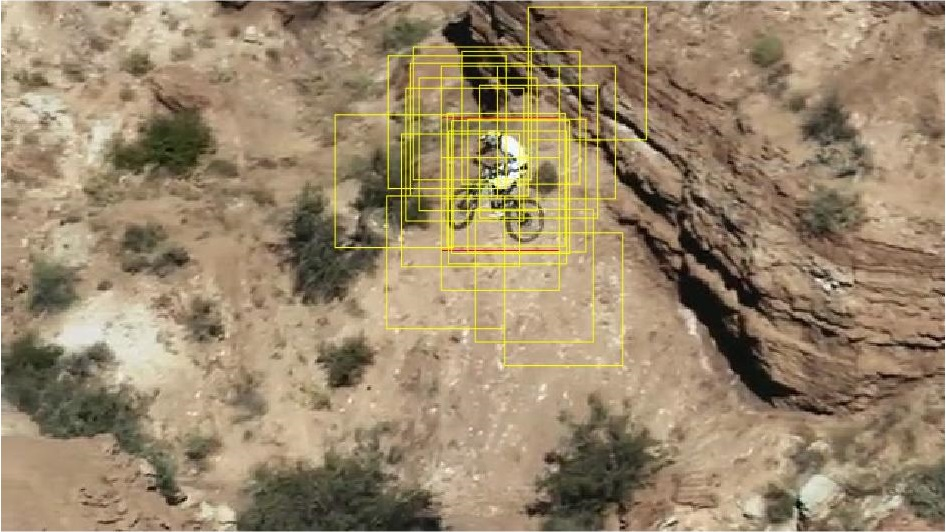
\includegraphics[width = 3in]{samples}
\caption{The location of the target from the previous frame (red box) and the normally sampled candidate patches (yellow boxes) for a biker from the video tracking dataset~\cite{wu2013online}.}
\label{fig:patches}
\end{figure}

\subsection{Computing Sample Features with a CNN}
For the next step of the algorithm, a CNN is used to transform each sample patch into a sample feature vector.
The CNN used should be pre-trained on a dataset for generic object detection in images; this is because CNNs trained for such a task have been known to create transformed representations of images useful for object discrimination~\cite{krizhevsky2012imagenet}.
Each candidate sample is passed through the CNN, and the output of the CNN's first fully-connected layer is used as the feature vector representing that sample.

The original algorithm by Hong, et al.~\cite{hong2015online} used the Caffe Model Zoo implementation of the pre-trained \textit{R-CNN} created by Girshick, et al.~\cite{girshick2016region} to create their sample feature vectors.
However,~\cite{hong2015online} specified in their paper that CNN models other than Girshick's R-CNN may also be used for similar results.
Thus, to circumvent the large amount of time needed to install Caffe, we decided to instead use MatConvNet~\cite{vedaldi2015matconvnet}, a CNN toolkit for Matlab with a simple installation process.
MatConvNet provides several pre-trained CNNs, and we decided to use \textit{VGG-F}, a CNN that has achieved state-of-the-art performance on the ImageNet object recognition database~\cite{chatfield2014return}.

\subsection{Using an SVM to Find Target-Specific Features from Sample Features}
Online SVM code has been acquired from Cauwenberghs, et al.~\cite{cauwenberghs2001incremental}. 
\todo

\subsection{Computing Class Saliency Maps}
Update this:
\todo
As one step of the algorithm, the target-specific features are back-propagated through the CNN in order to generate a target-specific saliency map, as detailed in~\cite{simonyan2013deep}.
This process involves taking the target-specific feature vector, inserting it into the first fully connected layer of the network, back-propagating this data to the input layer, and performing minor post-processing on this data.
Due to the process of back-propagation, the saliency maps are meant to highlight those pixels which have the most impact in identifying the  object in the image, effectively segmenting the foreground from the background.
A Matlab function was written to perform this operation.
Because the code to generate the target-specific features has not yet been written, this code currently takes as a parameter the sample features directly, which may include information about the background.
An example image with its corresponding saliency map is shown in Figure~\ref{fig:saliency}.
Note that the saliency map mostly highlights those pixels that correspond to the target foreground.

\begin{figure}[h]
\begin{tabular}{cc}
\subfloat[Original Image]{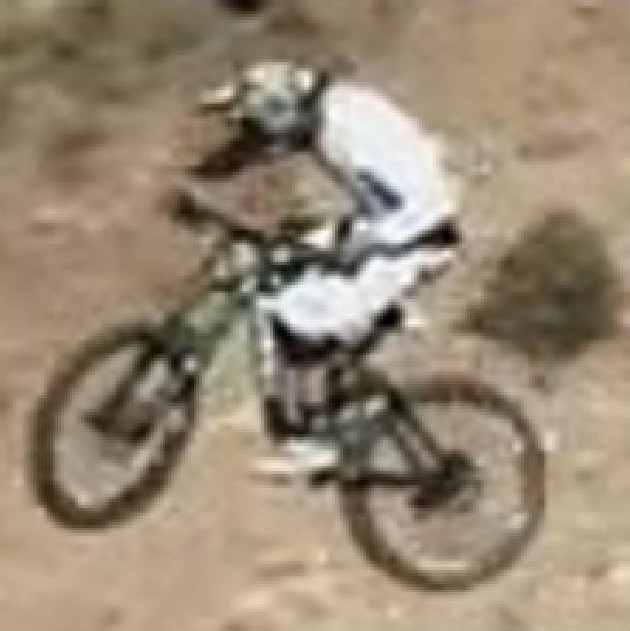
\includegraphics[width = 1.5in]{bike}}&
\subfloat[Saliency Map]{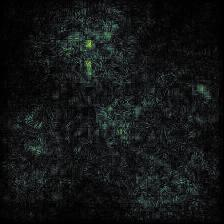
\includegraphics[width = 1.5in]{bike_saliency}}
\end{tabular}
\centering
\caption{The class saliency map for an image taken from the video tracking dataset used in this paper.}
\label{fig:saliency}
\end{figure}

\section{Work Distribution among Authors}
This section outlines how the work was distributed between the two authors of this report. 

\subsection{Aaron Gonzales}
\textit{Aaron Gonzales} was primarily responsible for generating the candidate sample patches, for using an SVM to find the target-specific features from the sample features, and training the online SVM.
He also researched the related work and was the primary contributor towards creating the Final Project presentation.

\subsection{Steven Hoffman}
\textit{Steven Hoffman} was primarily responsible for writing the skeleton code for the overall tracking algorithm, passing samples through the CNN to get the sample features, back-propagating the target-specific features through the CNN to create a target-specific saliency map, computing the generative model, and finding the target posterior.

\subsection{Both Authors}
\textit{Both authors} worked together to write up the various project reports, to give the final presentation, and to run the code on various testing sequences (i.e. videos).

\bibliography{proj-report}
\bibliographystyle{unsrt}
\end{document}
